\section{Results}
\label{sec:results}
\begin{figure}[htbp]
\vspace{-.3cm}
   \centering
    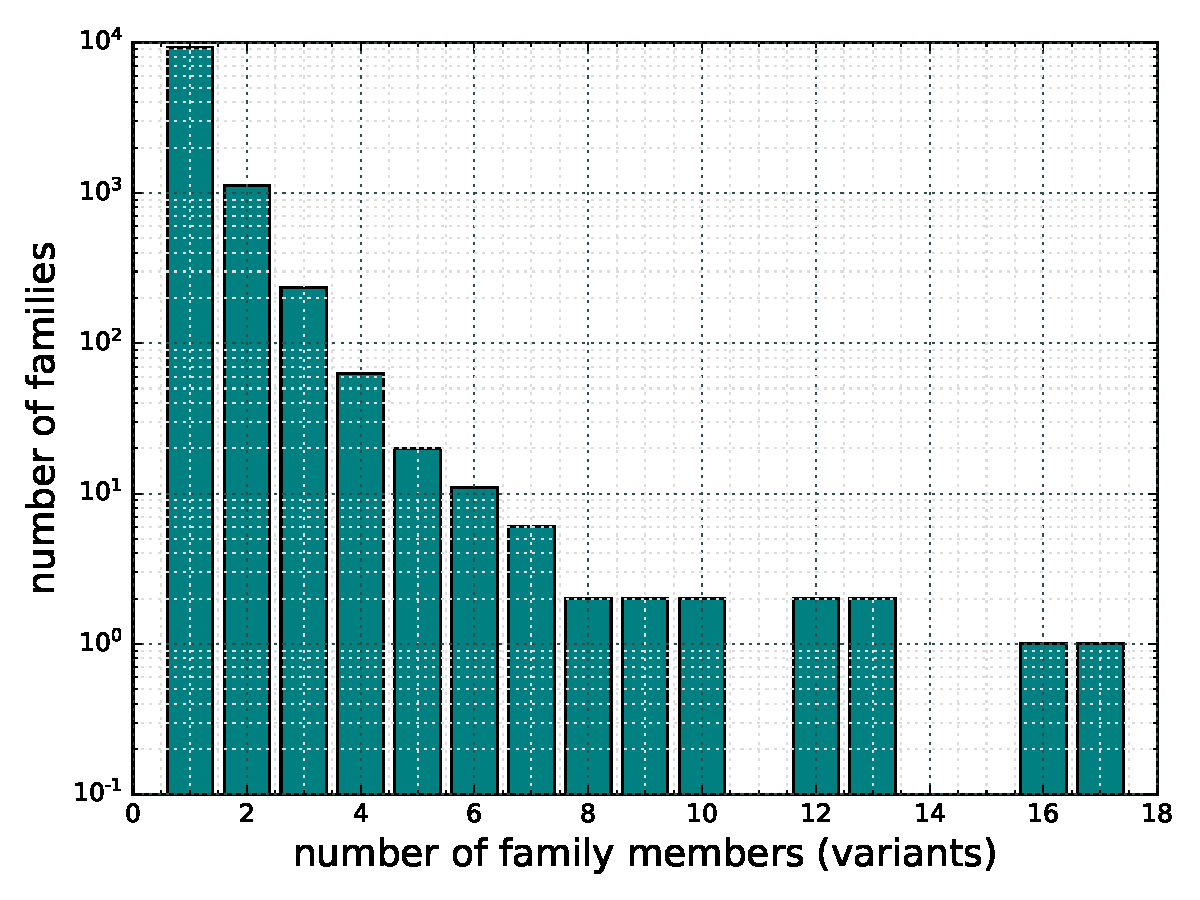
\includegraphics[scale=0.4]{figures/variants.pdf}
    \caption{Family size (number of variants in a family).}
   
    \label{fig:variants}
\end{figure}

\noindent
$RQ_0$: \textbf{How prevalent are software families in \js ecosystem on \gh?}

With this first RQ, we aim to determine if software families exist in software ecosystems. In the \js ecosystem we discovered a total 10,743 distinct mainlines and 12,813 variants in total. This means that we have a total of 10,743 software families. Figure~\ref{fig:variants} present a histogram of the distribution of the number of variants per mainline. The y-axis (in log-scale) shows the number of mainlines and  the x-axis shows the number of variants per mainline. For example, the first bar tells us that there are 9,280 mainlines that contain only one variant. We also observe two large mainlines containing 16 and 17 variants. The results of $RQ_0$ reveal that software families indeed exist in the \js ecosystem on \gh.%\tm{The last sentence is too generic. It only shows that software families exist in the \np-\gh ecosystem, nothing more.}

\begin{framed}
\noindent
\emph{We have identified a total 10,743 distinct mainlines and 12,813 variants in total. This gives us confidence that indeed software families exist in the \js ecosystem on \gh.}
\end{framed}

\begin{figure}[htbp]
\vspace{-.3cm}
   \centering
    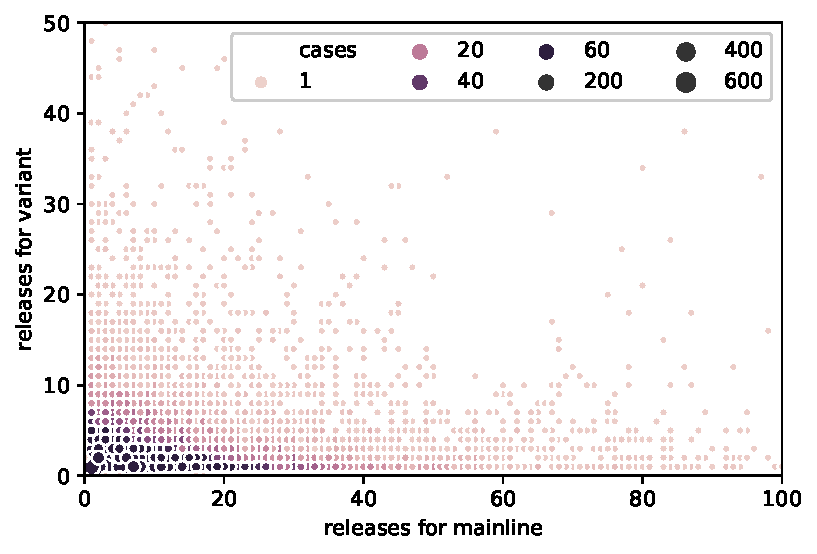
\includegraphics[scale=0.6]{figures/benevolj_releases.pdf}
    \caption{The distribution of the mainline versus variant package releases.}
    \label{fig:releases}
\end{figure}

%\tm{It would be nice to have a summary box at the end of each RQ}

$RQ_1$: \textbf{How do the distributions of package dependencies in mainlines and their variants compare to each other?}

With this second RQ, we aim to ascertain if the mainlines and the variants are continuously maintained. 
Figure~\ref{fig:releases} presents a scatter plot showing the distribution of releases for the variants versus the releases for the mainlines. 
On the x-axis we have the number of releases for the mainlines and on the y-axis we have the number of releases for the variants. 
The color of the data points in the graph represent the number cases for the mainlines\,/\,variants. 
For example, the data points on the top left of the graph tell us that there are some variants that have more releases compared to their mainline counterparts. 
This implies those specific variants are being maintained more than their mainline counterparts.
The data points on the bottom right tell us that there are a number of mainlines having many releases compared to their variant counterparts. 
Overall, we observe more mainlines being maintained compared to their variant counterparts.
However, we also observe a significant amount of variants being maintained. 
This is interesting since developers variants did not make a one off package distribution; they are continuously distributing new releases of their package. 

\begin{framed}
\noindent
\emph{We have observed that while many mainlines are being maintained more that their variant counterparts (which is not surprising), we do observe a significant number of variants being maintained \sd{in parallel}. Interestingly we have also observed quite a significant number of variants that are more \sd{actively} maintained than their mainline counterparts.}
\end{framed}

\begin{figure}[htbp]
\vspace{-.3cm}
   \centering
    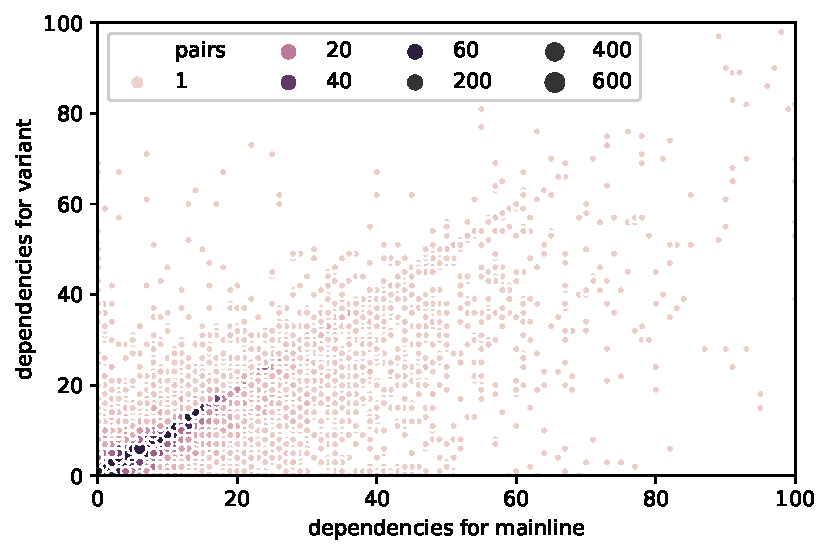
\includegraphics[scale=0.6]{figures/benevolj_dependencies.pdf}
    \caption{The distribution of the mainline versus variant package dependencies.}
    \label{fig:dependencies}
\end{figure}

%\tm{It would be nice to have a summary box at the end of each RQ}

$RQ_2$: \textbf{How do the distributions of package dependencies in mainlines and their variants compare to each other?}

With this RQ, we want to ascertain the frequency of package dependencies on other packages for the mainlines and the variants in the software families. 
Figure~\ref{fig:dependencies} presents a scatter plot showing the distribution of the package dependencies of the variants versus the dependencies of the mainline.
On the x-axis we have the number of dependencies of the mainline. 
On the y-axis we have the number of dependencies of the variant.
The color of the data points in the graph represent the number cases for the mainlines\,/\,variants.
For example, on the top right of the graph we see a few scattered points single case variants telling us that there are a few variants that have many dependencies compared to the mainline counterparts.
We also see many scattered single case mainlines having many dependencies compared to their variant counterparts. 
Overall, we observe the mainlines having more dependencies compared to their variant counterparts.

\begin{framed} 
\noindent
\emph{We have observed that although the mainlines have more dependencies on other packages compared to their variant counterparts, we do observe a significant number of variants that have dependencies.}
\end{framed}

\begin{figure*}[htbp]%
\vspace{-.3cm}
    \centering
    \subfloat[Packages]{{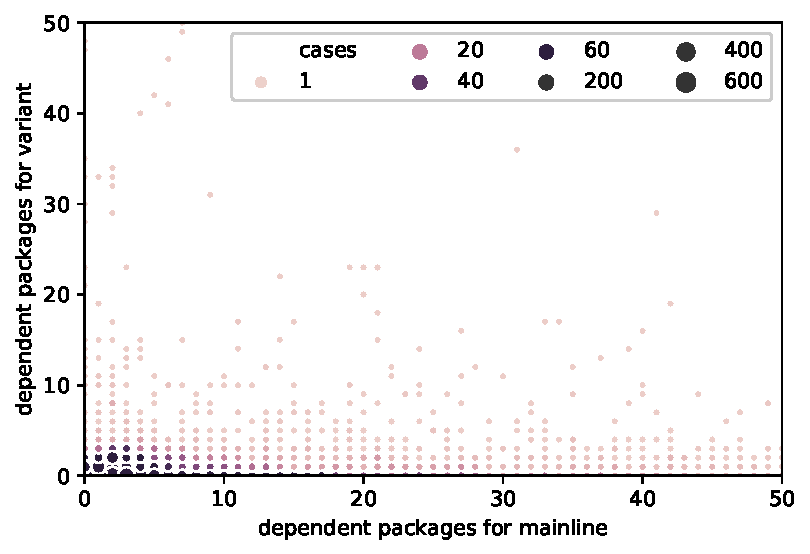
\includegraphics[width=8cm]{figures/dependents} }}%
    \qquad
    \subfloat[Projects]{{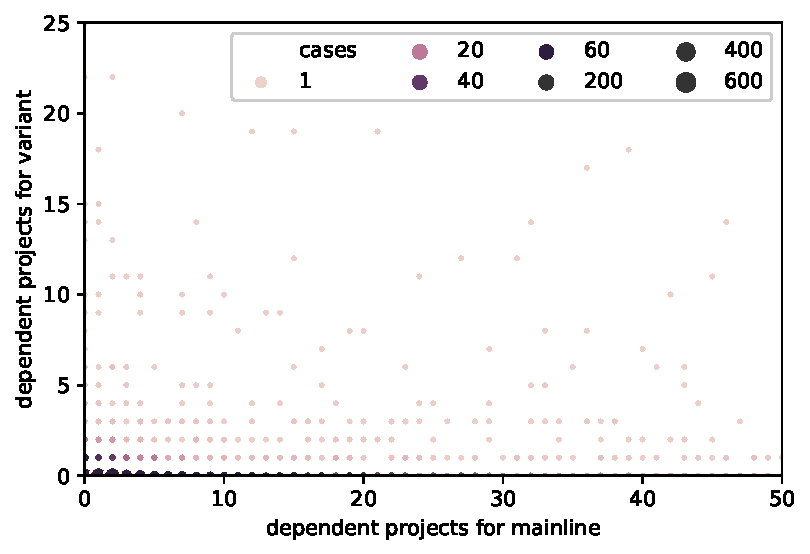
\includegraphics[width=8cm]{figures/benevolj_projects} }}%
    \caption{Distribution of dependent packages and dependent projects for the mainline versus variants.}%
    \label{fig:packages_and_projects}%
\end{figure*}

\begin{comment}
\begin{figure*}[htbp]%
\vspace{-.3cm}
    \centering
    \subfloat[ Mainlines]{{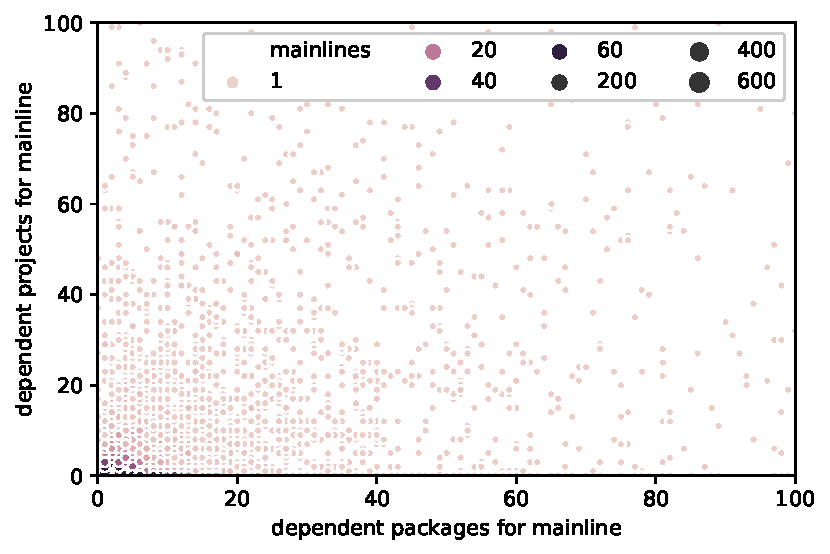
\includegraphics[width=8cm]{figures/benevolj_dependents_mainline.pdf} }}%
    \qquad
    \subfloat[ Variants]{{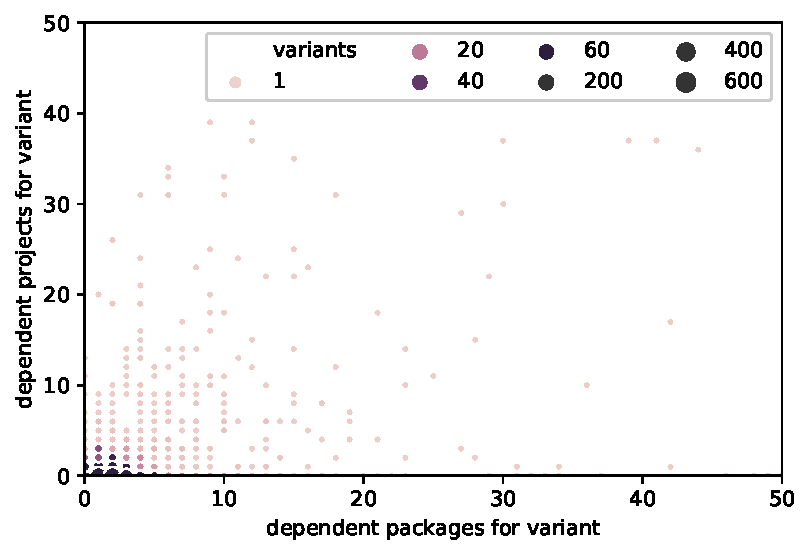
\includegraphics[width=8cm]{figures/benevolj_dependents_variant.pdf} }}%
    \caption{Distribution of dependent packages versus dependent projects for mainlines and variants.}%
    \label{fig:mainline_variants_packages}%
\end{figure*}
\end{comment}
%\tm{It would be nice to have a summary box at the end of each RQ}

$RQ_3$: \textbf{Do the variant projects have dependent packages\,/\,projects?}

In this RQ we are interesting in observing if other packages\,/\,projects in the ecosystem depend on the variants.
In Figure~\ref{fig:packages_and_projects} we present the scatter plots showing the distribution of the dependent packages (Figure~\ref{fig:packages_and_projects}-(a)) and dependent projects (Figure~\ref{fig:packages_and_projects}-(b)) for the variants versus mainlines.
The x-axes represent the number of dependent packages for the mainline and number of dependent projects for the variants, respectively.
The y-axes represent the number of dependent packages for the variants and number of dependent projects for the variants, respectively.
The color of the data points in the graph represent the number cases for the mainlines\,/\,variants.
Looking at Figure~\ref{fig:packages_and_projects}-(a), we observe that most of the data points are concentrated on the x-axis. 
This implies that there are very many mainline variants having many dependent packages compared to their variant counterparts.
We observe the same trend for the dependent projects in Figure~\ref{fig:packages_and_projects}-(b).
In both Figure~\ref{fig:packages_and_projects}-(a) and Figure~\ref{fig:packages_and_projects}-(b), we observe that most variants have $<10$ dependent packages\,/\,projects. 
This is still interesting since it implies that some developers do depend on the variants as opposed to their mainlines counterparts offering similar functionality. 
%In Figure~\ref{fig:mainline_variants_packages}-(a) we present a scatter plot showing the distribution of dependent projects of mainline vs the dependent packages of the mainline, while in Figure~\ref{fig:mainline_variants_packages}-(b) we show the same for variants. In both Figure~\ref{fig:mainline_variants_packages}-(a) and~\ref{fig:mainline_variants_packages}-(b) the y-axes represent the number of dependent projects for the mainlines\,/\,variants and the x-axes represent the number of dependent packages for the mainlines\,/\,variants, respectively. The color of the data points in the graphs represent the number cases for the mainlines\,/\,variants, respectively. We observe that the graph for the mainlines have more concentration of data points all over the graph compared the variants. this implies that the mainlines have more dependent packages/projects compared to the variants. However, irrespective of lower number of dependent packages/projects on the variants, it is still interesting to see some variants hanging dependents.

\begin{framed}
\noindent
\emph{We have observed that the compared to the mainline counterparts, the variant have fewer dependent packages/projects. Since it is plausible to assume that the mainline and variants offer similar functionality because of the common code base, it is still interesting to observe that other projects using the variants package releases.}
\end{framed}
